%%%%%%%%%%%%%%%%%%%%%%%%%%%%%%%%%%%%%%%%%%%%%%%%%%%%%%%%%%%%%%%%%%%%%%%%%%%%%%%%%%%%%%%%%%%%%%%%%%%%%%%%%%%%%%%%%%%%%%%%%%%%%%%
%%     LaTeX Dokumentvorlage
%%     für Diplomarbeiten an der HTL Hollabrunn
%%     ---------------------------------------------------------------------
%%     für Verwendung mit
%%     - biblatex und biber
%%     - UTF8
%%     - TeX-Studio
%%     - siunitx - Paket
%%
%%     Installation unter Windows: erst MiKTeX und *dann* TeX-Studio installieren, fertig
%%%%%%%%%%%%%%%%%%%%%%%%%%%%%%%%%%%%%%%%%%%%%%%%%%%%%%%%%%%%%%%%%%%%%%%%%%%%%%%%%%%%%%%%%%%%%%%%%%%%%%%%%%%%%%%%%%%%%%%%%%%%%%%

%%%%%%%%%%%%%%%%%%%%%%%%%%%%%%%%%%%%%%%%%%%%%%%%%%%%%%%%%%%%%%%%%%%%%%%%%%%%%%%%%%%%%%%%%%%%%%%%%%%%%%%%%%%%%%%%%%%%%%%%%%%%%%%
%%     LaTeX Präambel für die Dokumentvorlage
%%     für Diplomarbeiten an der HTL Hollabrunn
%%     ---------------------------------------------------------------------
%%     !!  HIER BITTE NICHTS ÄNDERN, außer Sie wissen genau, was Sie tun  !! Wir wissen es
%%%%%%%%%%%%%%%%%%%%%%%%%%%%%%%%%%%%%%%%%%%%%%%%%%%%%%%%%%%%%%%%%%%%%%%%%%%%%%%%%%%%%%%%%%%%%%%%%%%%%%%%%%%%%%%%%%%%%%%%%%%%%%%

\documentclass[a4paper,11pt,DIV15,oneside,normalheadings,headsepline,twoside]{scrreprt}
									% mit chapter, section, subsection, subsubsection
%\documentclass[a4paper,12pt,DIV15,oneside,normalheadings,headsepline]{scrartcl}
									% mit section, subsection, subsubsection
% ------------------------------------------------------------------------------------------------------------

% -----------------PAKETE (löschen/hinzugeben nur, wenn man sich sicher ist) -------------------------------------
\usepackage[utf8]{inputenc}		    % damit die Tastatur richtig erkannt wird (passt immer, egal welches OS)
\usepackage{lmodern}
\usepackage[T1]{fontenc} 			% europäische Schrifttypen, wichtig für Copy&Paste aus pdf
\usepackage{textcomp}				% Sonderzeichen wie in l2kurz , S.45
\usepackage{color}

\usepackage[austrian]{babel}		% Abteilungen usw. \usepackage{german} beisst sich mit gnuplottex
\usepackage[style=trad-unsrt, backend=biber]{biblatex}
\usepackage{hyperref}
\definecolor{darkblue}{rgb}{0,0,0.845}
\hypersetup{colorlinks=true, citecolor=darkblue, urlcolor=darkblue, linkcolor=darkblue}
\usepackage{url}
	% macht die URL im Literaturverzeichnis hübscher
	\DeclareFieldFormat{url}{\newline\mkbibacro{URL}\addcolon\nobreakspace\url{#1}}
\usepackage{breakurl}
% \usepackage[automark]{scrlayer-scrpage}
\usepackage[left=2.2cm, right=1.5cm, top=3cm, bottom=4.5cm]{geometry}
\usepackage{amsmath,amssymb,amsfonts,textcomp}  % Mathegeschichten und Symbole
\usepackage{wasysym,latexsym}      	% für \Smiley und \Frowny,...
\usepackage[right]{eurosym}			% für \euro{} oder \EUR{53,15} Opt. left/right, jenachdem, ob 53,15€ oder €53,15
\usepackage{makecell}
\usepackage{lipsum}
\usepackage{float}               	% einfacher Weg, um Abb. zu fixieren mit [H]
\usepackage{nonfloat}
%\usepackage[scanall]{psfrag}        % Ersetzen von Text in Abbildungen (geht *nicht* mit pdfLaTeX)
\usepackage{lscape, pdflscape}      % soll Tabellen im Landscape-Format im Reader
									% automatisch drehen, sonst wie landscape
\usepackage{overpic}				% reinschreiben in ein Bild, Koordinaten jeweils von 0-100
\usepackage{subfigure}				% \subfigure{\includegraphics[...]{...}}
									% \subfigure{\includegraphics[...]{...}} <- mehrere Abb. in einer figure
%\usepackage[shell]{gnuplottex}
%\usepackage{pdfsync}				% für das Springen aus dem PDF in den Editor, nicht mehrnotwendig
\usepackage{graphicx} 		        % ohne genauere Spezifizierung in eckigen Klammern
\usepackage{setspace}				% für Anderung des Zeilenabstandes

%\usepackage[basic]{circ}

\usepackage{listings}				% Einbinden von Quellcode
\usepackage{pst-pdf, pstcol, pst-osci}

\usepackage{epstopdf}				% Beim kompilieren wird on the fly ein 	*.pdf erstellt.

%\usepackage[thickspace,thickqspace,squaren]{SIunits}
\usepackage{siunitx}
\sisetup{locale = DE}

\usepackage{fancyhdr}
\usepackage{titlesec}
\usepackage{pdfpages}


\titleformat{\chapter}
{\normalfont\Huge\bfseries}{\thechapter}{1em}{}
\titleformat{\section}
{\normalfont\huge\bfseries}{\thesection}{1em}{}
\titleformat{\subsection}
{\normalfont\LARGE\bfseries}{\thesubsection}{1em}{}
\titleformat{\subsubsection}
{\normalfont\LARGE\bfseries}{\thesubsubsection}{1em}{}


%---------------------------------- EINTRAEGE fuer  LAYOUT (evtl. anpassen)   -----------------------------------
% Disable single lines at the start of a paragraph (Schusterjungen)
\clubpenalty = 10000
%
% Disable single lines at the end of a paragraph (Hurenkinder)
\widowpenalty = 10000 \displaywidowpenalty = 10000
%

%-------------------------------------------------------------------------------
% Erstellt die Header und Footer der Seiten mit Autor pro Seite
% Wenn nicht zweiseitig ([OL,OR], ...) anpassen
%-------------------------------------------------------------------------------
\fancypagestyle{alle}{
	\fancyhf{}
	\fancyhead[EL,OR]{\rightmark}
	\fancyfoot[OL,ER]{HTBL Hollabrunn}
	\fancyfoot[C]{\schuelerAlle}
	\fancyfoot[EL,OR]{\thepage}
	\renewcommand{\headrulewidth}{0.3pt}
	\renewcommand{\footrulewidth}{0.3pt}
}

\fancypagestyle{plain}[alle]{
	\fancyfoot[C]{}
}

\fancypagestyle{SchuelerA}[alle]{
	\fancyfoot[C]{\schuelerA}
}

\fancypagestyle{SchuelerB}[alle]{
	\fancyfoot[C]{\schuelerB}
}

\fancypagestyle{SchuelerC}[alle]{
	\fancyfoot[C]{\schuelerC}
}


\fancypagestyle{SchuelerD}[alle]{
	\fancyfoot[C]{\schuelerD}
}

\renewcommand{\chaptermark}[1]{\markright{\thechapter\ #1}}
\renewcommand{\sectionmark}[1]{\markright{\thesection\ #1}}
%\renewcommand{\subsectionmark}[1]{\markright{\thesubsection\ #1}}
%\renewcommand{\subsubsectionmark}[1]{\markright{\thesubsubsection\ #1}}

%\sectionfont{\fontsize{12}{15}\selectfont}
%\subsectionfont{\fontsize{12}{15}\selectfont}
%\subsubsectionfont{\fontsize{12}{15}\selectfont}
\renewcommand\lstlistlistingname{Code-Verweise}

\parindent0em							% Einzug bei neuen Absätzen
\parskip1mm								% Abstand zwischen Absätzen
\sloppy									% nicht soooo genau mit dem Blocksatz
% ---------------------------------------------------------------------------------------------------------------
\def\schuelerEmpty{~}

% ------------------------------------------------------------------------------------------------------		% NICHT löschen
%%%%%%%%%%%%%%%%%%%%%%%%%%%%%%%%%%%%%%%%%%%%%%%%%%%
%%                   anpassen....                %%
%%%%%%%%%%%%%%%%%%%%%%%%%%%%%%%%%%%%%%%%%%%%%%%%%%%
%---------------------------------------- GRAPHIKPFAD (***anpassen***)  -----------------------------------------
% gleiches Verzeichnis oder Unterordner Bilder, auch absolute Pfade, NIE Backslash, CASE-sensitive!!!!
\graphicspath
{
	{./}
	{./img/}
}
\def\schuelerA{Schüler A}
\def\schuelerB{Schüler B}				% nicht weglöschen sondern \def\schuelerB{~}
\def\schuelerC{Schüler C}           % nicht weglöschen sondern \def\schuelerC{~}
\def\schuelerD{Schüler D}          % nicht weglöschen sondern \def\schuelerD{}

\newcommand{\schuelerAlle}{A, B, C, D}

\newcommand{\betreuerA}{Betreuer A}
\newcommand{\betreuerB}{}       % nicht weglöschen sondern zB \newcommand{\betreuerB}{}

\newcommand{\schuljahr}{JJJJ/JJ}
\newcommand{\daTitel}{DA Titel lang}
\newcommand{\daTitelKurz}{DA Titel kurz}
\newcommand{\datumErklaerung}{TT.MM.JJJJ}			% Datum für die eidesstattliche Erklärung
\newcommand{\datumAbgabe}{TT.MM.JJJJ}
\newcommand{\aktuellesSchuljahr}{JJJJ/JJ}	% Enthält alle Definiotinen wie Schüler und Betreuer
\addbibresource{my_library.bib}
%%%%%%%%%%%%%%%%%%%%%%%%%%%%%%%%%%%%%%%%%%%%%%%%%%%%%%%%%%%%%%%%%%%%%%%%%%%%%%%%%%%%%%%%%%%%%%%%%%%%%%%%%%%%%%%%%%%%%%%%%%%%%%%
%%   unbedingt in TeX-Studio Optionen->TeX-Studio konfigurieren->Erzeugen->Standardbibliographieprogramm "Biber" einstellen  %%
%%%%%%%%%%%%%%%%%%%%%%%%%%%%%%%%%%%%%%%%%%%%%%%%%%%%%%%%%%%%%%%%%%%%%%%%%%%%%%%%%%%%%%%%%%%%%%%%%%%%%%%%%%%%%%%%%%%%%%%%%%%%%%%

%%%%%%%%%%%%%%%%%%%%%%%%%%%%%%%%%%%%%%%%%%%%%%%%%%%%%%%%%%%%%%%%%%%%%%%%%%%%%%%%%%%%%%%%%%%%%%%%%%%%%%%%%%%%%%%%%%%%%%%%%%%%%%%
%%                    falsche / unglückliche Abteilungen kann man hier für das ganze Dokument verändern                      %%
%%                    zB  Di-plomarbeit oder Diplomar-beit statt Diplom-arbeit                                               %%
%%%%%%%%%%%%%%%%%%%%%%%%%%%%%%%%%%%%%%%%%%%%%%%%%%%%%%%%%%%%%%%%%%%%%%%%%%%%%%%%%%%%%%%%%%%%%%%%%%%%%%%%%%%%%%%%%%%%%%%%%%%%%%%
\hyphenation{Diplom-arbeit}
\hyphenation{En-ti-ty-Stu-dent-Has-Assign-ment}


%%%%%%%%%%%%%%%%%%%%%%%%%%%%%%%%%%%%%%%%%%%%%%%%%%%%%%%%%%%%%%%%%%%%%%%%%%%%%%%%%%%%%%%%%%%%%%%%%%%%%%%%%%%%%%%%%%%%%%%%%%%%%%%
%                                         an ihre Teil-Dokumente anpassen                                                    %%
%%%%%%%%%%%%%%%%%%%%%%%%%%%%%%%%%%%%%%%%%%%%%%%%%%%%%%%%%%%%%%%%%%%%%%%%%%%%%%%%%%%%%%%%%%%%%%%%%%%%%%%%%%%%%%%%%%%%%%%%%%%%%%%
\begin{document}
	\pagestyle{alle}
	\definecolor{commentgreen}{RGB}{10,126,18}
\lstdefinestyle{bashStyle}{
	language     = bash,
	showstringspaces=false,
	frame=single,
	rulecolor=\color{black},
	inputencoding=utf8,
	basicstyle   = \footnotesize\ttfamily,
	keywordstyle = \color{blue},
	commentstyle = \color{commentgreen},
	stringstyle  = \color{orange},
	tabsize      = 4,
	captionpos   = b,
	breaklines=true,
	numbers=left,
	backgroundcolor=\color{gray!10!white},
	literate=
		{Ö}{{\"O}}1
		{Ä}{{\"A}}1
		{Ü}{{\"U}}1
		{ß}{{\ss}}1
		{ü}{{\"u}}1
		{ä}{{\"a}}1
		{ö}{{\"o}}1
}


\lstdefinelanguage{kotlin}{
	morekeywords={fun, interface, data, class, val, return, enum, var},
	morecomment=[s]{/**}{*/}
	%morestring=[b]"
}
\lstdefinestyle{kotlinStyle}{
	language     = kotlin,
	showstringspaces=false,
	frame=single,
	rulecolor=\color{black},
	inputencoding=utf8,
	basicstyle   = \footnotesize\ttfamily,
	keywordstyle = \color{blue},
	commentstyle = \color{commentgreen},
	stringstyle  = \color{orange},
	tabsize      = 4,
	captionpos   = b,
	breaklines=true,
	numbers=left,
	backgroundcolor=\color{gray!10!white}
}  			% Einbinden von Quellcode, muss für andere Sprachen als bash, muss angepasst werden
	
	%%%%%%%%%%%%%%%%%%%%%%%%%%%%%%%%%%%%%%%%%%%%%%%%%%%
    %%            hier nichts ändern                 %%
    %%%%%%%%%%%%%%%%%%%%%%%%%%%%%%%%%%%%%%%%%%%%%%%%%%%	
	
	\newgeometry{top=2cm,left=2cm,right=2cm}
	\begin{titlepage}
		
		\begin{center}
			\begin{tabular}{ c c c }
				\thead{
\includegraphics[width=33mm]{htlhl_bildung_mit_zukunft}} &
				\thead{\Large{\textbf{HTBL Hollabrunn}} \\ \small{\textbf{Höhere Lehranstalt für Informationstechnologie}}} &
				\thead{
\includegraphics[width=21mm]{htlhl_logo}}
			\end{tabular}
			
			\vspace{40mm}
			
			\Huge{\textbf{Diplomarbeit}}
		    
		    \vspace{10mm}
		    
			\Huge{\textbf{\daTitel}}	 
		\end{center}
		
		\vspace{20mm}	% Hier könnte eine Abbildung gut aussehen
		
		\begin{large}
			\begin{tabular}{p{25mm}p{100mm}}
			 Verfasser: &  \schuelerA	\\
			            &  \schuelerB	\\
			            &  \schuelerC	\\
			            &  \schuelerD	\\
			 ~			& 				\\
			 Betreuer:  & \betreuerA	\\
			 		    & \betreuerB  	\\ 
			\end{tabular} 
		\end{large}
		
		\vspace{20mm}
		
		\begin{large}
			Schuljahr: \aktuellesSchuljahr
			~ \\
			~ \\
			\rule{\textwidth}{1.0pt} \\
			~ \\
			Abgabevermerk: \\
			~ \\
			~ \\
			Datum: \datumAbgabe \qquad \qquad \qquad übernommen von:
		\end{large}
		
	\end{titlepage}
	\newpage\null\thispagestyle{empty}\newpage % Irgendwie ganz leere Seite, ka
	\begin{center}
	\hfill
	
\includegraphics[width=30mm]{htlhl_logo} \\
	\vspace{10mm}
	\huge{\textbf{Höhere Technische Bundeslehranstalt Hollabrunn}} \\
	\large{\textbf{Höhere Lehranstalt für Informationstechnologie}} \\
\end{center}

\vspace{10mm}

\large{EIDESSTATTLICHE ERKLÄRUNG} \\
Ich erkläre an Eides statt, dass ich die vorliegende Diplomarbeit selbständig und ohne fremde Hilfe verfasst, andere als die angegebenen Quellen und Hilfsmittel nicht benutzt und die den benutzten Quellen wörtlich und inhaltlich entnommenen Stellen als solche erkenntlich gemacht habe.


\vspace{25mm}
\rule{\textwidth}{1.0pt}
Hollabrunn, am \datumErklaerung , \schuelerA


\if \schuelerB \schuelerEmpty
	~
\else
	\vspace{15mm}
	\rule{\textwidth}{1.0pt}
	Hollabrunn, am \datumErklaerung , \schuelerB
\fi


\if \schuelerC \schuelerEmpty
	~
\else
	\vspace{15mm}
	\rule{\textwidth}{1.0pt}
	Hollabrunn, am \datumErklaerung , \schuelerC
\fi


\if \schuelerD \schuelerEmpty
    ~
\else
	\vspace{15mm}
	\rule{\textwidth}{1.0pt}
	Hollabrunn, am \datumErklaerung , \schuelerD
\fi

	\newpage\null\thispagestyle{empty}\newpage
	\chapter*{HINWEISE}
\markright{Hinweise}

Die vorliegende Diplomarbeit wurde in Zusammenarbeit mit der Firma ..... ausgeführt. \\
~ \\
oder \\
~ \\
Die vorliegende Diplomarbeit wurde für die Abteilung Informationstechnologie der HTL Hollabrunn ausgeführt. \\
~ \\
Die in dieser Diplomarbeit entwickelten Prototypen und Software-Produkte dürfen ganz oder auch in Teilen von Privatpersonen oder Firmen nur dann in Verkehr gebracht werden, wenn sie diese selbst geprüft und für den vorgesehenen Verwendungszweck für geeignet befunden haben.
Es wird keinerlei Haftung übernommen für irgendwelche Schäden, die aus der Nutzung der hier entwickelten oder beschriebenen Bestandteile des Projekts resultieren. \\
~ \\
Für alle Entwicklungen gilt die GNU General Public License \verb|[http://www.gnu.org/licenses/gpl.html]| der Free Software Foundation, Boston, USA in der Version 3. \\
~ \\
Absatz überarbeiten bzw. Rundschreiben aktualisieren!
Die Diplomarbeit erfüllt die “Standards für Ingenieur- und Technikerprojekte” entsprechend dem Rundschreiben Nr. 60 aus 1999 des BMBWK (GZ.17.600/101-II/2b/99).
\verb|[https://www.bmb.gv.at/ministerium/rs/1999_60.html]|

	\chapter*{SCHLÜSSELBEGRIFFE}
\markright{Schlüsselbegriffe}

	\chapter*{DANKSAGUNGEN}
\markright{Danksagungen}
\vspace{-1cm} % Boss move
Danke, danke, danke.

\newpage
	\markright{}
	% Kurzfassung
\begin{center}
	\begin{table}[h!]
		\begin{tabular}{|c|c|}
			\hline
			\thead{
\includegraphics[width=33mm]{htlhl_bildung_mit_zukunft}} &
			\thead{{\textbf{HÖHERE TECHNISCHE BUNDESLEHRANSTALT HOLLABRUNN}} \\\hline \\ \Large{\textbf{Informationstechnologie}}}\\
			\hline
		\end{tabular}
	\end{table}
	~ \\
	~ \\
	\Huge{\textbf{DIPLOMARBEIT}}\\
	\LARGE{\textbf{DOKUMENTATION}}
	~ \\
	~ \\
	\begin{table}[h!]
		\begin{tabular}{|p{50mm}|p{110mm}|}
			\hline
			\thead{Name der \\ Verfasser/innen} &
			\thead{\schuelerA, \schuelerB, \\ \schuelerC, \schuelerD} \\
			\hline
			\thead{Jahrgang \\ Schuljahr} &
			\thead{\aktuellesSchuljahr} \\
			\hline
			\thead{Thema der Diplomarbeit} &
			\thead{\daTitel} \\
			\hline
			\thead{Kooperationspartner} &
			\thead{} \\
			\hline
		\end{tabular}
	\end{table}
	\begin{table}[h!]
		\begin{tabular}{|p{50mm}|p{110mm}|}
			\hline
			\makecell[l{{p{50mm}}}]{\small{Aufgabenstellung}} &
			\makecell*[{{p{110mm}}}]{\small{Blub}} \\
			\hline
		\end{tabular}
	\end{table}
	\begin{table}[h!]
		\begin{tabular}{|p{50mm}|p{110mm}|}
			\hline
			\makecell[l{{p{50mm}}}]{\small{Realisierung}} &
			\makecell*[{{p{110mm}}}]{\small{Blub}} \\
			\hline
		\end{tabular}
	\end{table}
	\begin{table}[h!]
		\begin{tabular}{|p{50mm}|p{110mm}|}
			\hline
			\makecell[l{{p{50mm}}}]{\small{Ergebnisse}} &
			\makecell*[{{p{110mm}}}]{\small{Blub}} \\
			\hline
		\end{tabular}
	\end{table}

	\newpage

	\begin{table}[h!]
		\begin{tabular}{|p{50mm}|p{110mm}|}
			\hline
			\makecell[l{{p{50mm}}}]{\small{Typische Grafik, Foto etc.(mit Erläuterung)}} &
			\makecell*[{{p{110mm}}}]{\vspace{3mm} 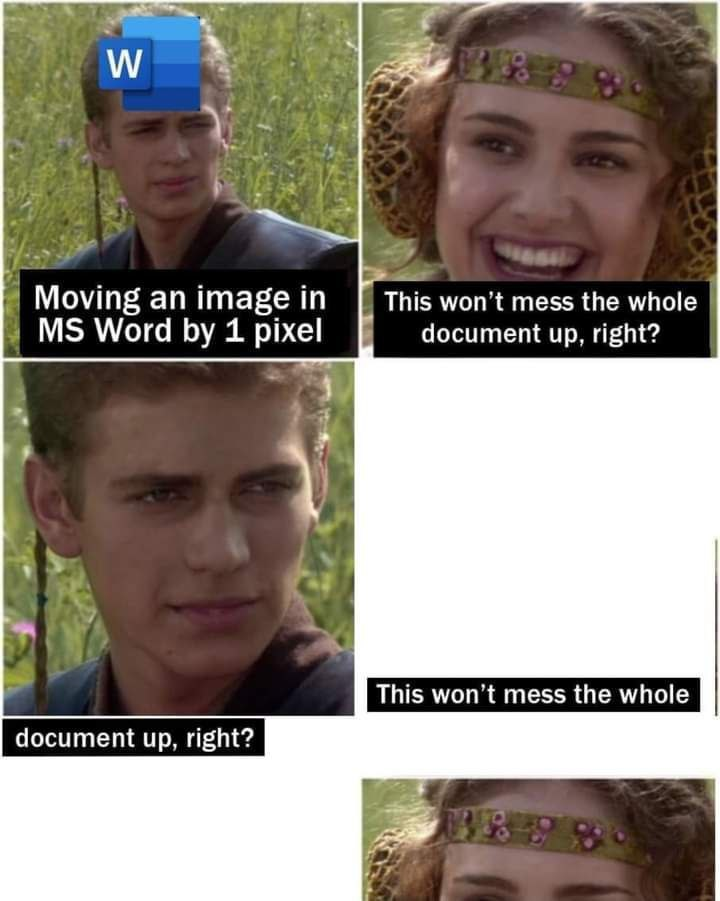
\includegraphics[width=110mm]{/img/word_meme2.jpeg} \vspace{3mm}} \\ % vspcae so anpassen dass sich alles auf einer Seite ausgeht
			\hline
		\end{tabular}
	\end{table}
	\begin{table}[h!]
		\begin{tabular}{|p{50mm}|p{110mm}|}
			\hline
			\makecell[l{{p{50mm}}}]{\small{Teilnahme an Wettbewerben, Auszeichnungen}} &
			\makecell*[{{p{110mm}}}]{\small{Blub}} \\
			\hline
		\end{tabular}
	\end{table}
	\begin{table}[h!]
		\begin{tabular}{|p{50mm}|p{110mm}|}
			\hline
			\makecell[l{{p{50mm}}}]{
				\small{Möglichkeiten der}\\
				\small{Einsichtnahme in die Arbeit}} &
			\makecell*[{{p{110mm}}}]{
				\small{HTL HollabrunnAnton} \\
				\small{Ehrenfriedstraße 10} \\
				\small{2020 Hollabrunn}} \\
			\hline
		\end{tabular}
	\end{table}
	\begin{table}[h!]
		\begin{tabular}{|p{52mm}|p{52mm}|p{52mm}|}
			\hline
			\makecell[l{{p{52mm}}}]{
				\small{Approbation} \\
				\small{(Datum / Unterschrift)} \\ ~ \\ ~ \\ ~ \\} &
			\makecell[l{{p{52mm}}}]{\small{Prüfer/Prüferin} \\ ~ \\ ~ \\ ~ \\ ~ \\} &
			\makecell[l{{p{52mm}}}]{
				\footnotesize{Direktor/Direktorin} \\
				\footnotesize{Abteilungsvorstand/} \\
				\footnotesize{Abteilungsvorständin}\\ ~ \\ ~ \\} \\
			\hline
		\end{tabular}
	\end{table}
\end{center}

\newpage
	% Abstract
\begin{center}
	\begin{table}[h!]
		\begin{tabular}{|c|c|}
			\hline
			\thead{
\includegraphics[width=33mm]{htlhl_bildung_mit_zukunft}} &
			\thead{
				\textbf{HÖHERE TECHNISCHE BUNDESLEHRANSTALT HOLLABRUNN} \\
				\textbf{COLLEGE of ENGINEERING } \\
				\hline \\
				\Large{\textbf{Information Technology}}} \\
			\hline
		\end{tabular}
	\end{table}
	~ \\
	~ \\
	\Huge{\textbf{DIPLOMA THESIS}}\\
	\LARGE{\textbf{Documentation}}
	~ \\
	~ \\
	\begin{table}[h!]
		\begin{tabular}{|p{50mm}|p{110mm}|}
			\hline
			\thead{Author(s)} &
			\thead{\schuelerA, \schuelerB, \\ \schuelerC, \schuelerD} \\
			\hline
			\thead{From \\ Academic year} &
			\thead{\aktuellesSchuljahr} \\
			\hline
			\thead{Topic} &
			\thead{\daTitel} \\
			\hline
			\thead{Co-operation partners} &
			\thead{} \\
			\hline
		\end{tabular}
	\end{table}
	\begin{table}[h!]
		\begin{tabular}{|p{50mm}|p{110mm}|}
			\hline
			\makecell[l{{p{50mm}}}]{\small{Assignment of tasks}} &
			\makecell*[{{p{110mm}}}]{\small{Blub}} \\
			\hline
		\end{tabular}
	\end{table}
	\begin{table}[h!]
		\begin{tabular}{|p{50mm}|p{110mm}|}
			\hline
			\makecell[l{{p{50mm}}}]{\small{Realisation}} &
			\makecell*[{{p{110mm}}}]{\small{Blub}} \\
			\hline
		\end{tabular}
	\end{table}
	\begin{table}[h!]
		\begin{tabular}{|p{50mm}|p{110mm}|}
			\hline
			\makecell[l{{p{50mm}}}]{\small{Results}} &
			\makecell*[{{p{110mm}}}]{\small{Blub}} \\
			\hline
		\end{tabular}
	\end{table}

	\newpage

	\begin{table}[h!]
		\begin{tabular}{|p{50mm}|p{110mm}|}
			\hline
			\makecell[l{{p{50mm}}}]{\small{Illustrative graph, photo (incl. explanation)}} &
			\makecell*[{{p{110mm}}}]{\vspace{3mm} 
\includegraphics[width=110mm]{word_meme1.png} \vspace{3mm}} \\ % vspcae so anpassen dass sich alles auf einer Seite ausgeht
			\hline
		\end{tabular}
	\end{table}

	\begin{table}[h!]
		\begin{tabular}{|p{50mm}|p{110mm}|}
			\hline
			\makecell[l{{p{50mm}}}]{\small{Participation in competitions Awards}} &
			\makecell*[{{p{110mm}}}]{\small{Blub}} \\
			\hline
		\end{tabular}
	\end{table}
	\begin{table}[h!]
		\begin{tabular}{|p{50mm}|p{110mm}|}
			\hline
			\makecell[l{{p{50mm}}}]{
				\small{Accessibility of}\\
				\small{final project thesis}} &
			\makecell*[{{p{110mm}}}]{
				\small{HTL HollabrunnAnton} \\
				\small{Ehrenfriedstraße 10} \\
				\small{2020 Hollabrunn}} \\
			\hline
		\end{tabular}
	\end{table}
	\begin{table}[h!]
		\begin{tabular}{|p{52mm}|p{52mm}|p{52mm}|}
			\hline
			\makecell[l{{p{52mm}}}]{\small{Approval (Date / Signature)} \\ ~ \\ ~ \\} &
			\makecell[l{{p{52mm}}}]{\small{Examiner/s} \\ ~ \\ ~ \\} &
			\makecell[l{{p{52mm}}}]{\small{Head of Department / College} \\ ~ \\ ~ \\} \\
			\hline
		\end{tabular}
	\end{table}
\end{center}

\newpage
	\newpage\null\thispagestyle{empty}\newpage
%	\includepdf[pages=-]{ABA_Erklaerung.pdf} 	% Anpassen

	\tableofcontents			% Erstellen des Inhaltsverzeichnisses
	\newpage
	\chapter{Einleitung}
	\section{Motivation für die Arbeit}
		\lipsum[1-1]
	\section{Umfeld, Stand der Technik}
		\lipsum[1-1]
	\section{Aufgabenstellung}
		\lipsum[1-1]

		\subsection{Ziele}
			\begin{itemize}
				\item Schritt 1
				\item Schritt 2
				\item Schritt 3
			\end{itemize}


		\subsection{Nicht-Ziele}
			\lipsum[1-1]
	% !TeX spellcheck = de_AT-GermanAustria
\chapter{Bewertungssystem} \label{sec:bewertungssystem}
\pagestyle{SchuelerA} % anpassen in praeambel und rein schreiben
\section{Section 1}
\lipsum[3-4]
\subsection{Subsection}
\lipsum[2-3]
\begin{figure}[th!]
	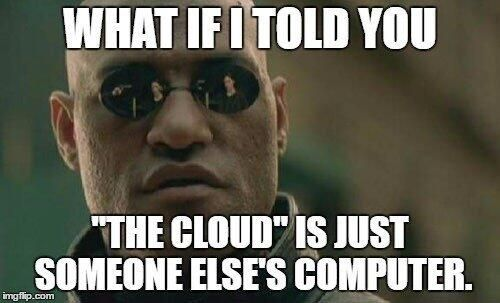
\includegraphics[width=\textwidth]{img/cloud_meme.jpg}
	\caption{Meme}
\end{figure}
\subsubsection{subsubsection}
	\lipsum[1-2]
\newpage
\subsection{Code Listing}
	Hier referiere ich auf das Code Listing: \ref{bash_script}
	\lstinputlisting[style=bashStyle, firstline=1, caption=Bash Script, label=bash_script]{./software/bashScript.sh}
	\pagestyle{alle}
	\chapter{Kurze Einf"uhrung in \LaTeX}
    F"ur die Diplomarbeit bitte dieses Kapitel im Masterdokument
    einfach auskommentieren (\%~davor).

	\LaTeX{} ist eine sehr leistungsf"ahige Software zum Verfassen wissenschaftlicher Arbeiten.

	Wichtige \LaTeX{}-Infos findet man in \cite{l2kurz}.

	\section{Gliederung (ich bin eine "Uberschrift -- section)}
	Ein neues Kapitel beginnt mit dem \verb|\chapter {Kapitelname}|-Befehl, z.\,B. die Kapitelüberschrift auf dieser Seite (Kurze Einführung \dots).

	Weitere Gliederungen sind:\\
	\verb|\section{Titel}|, \verb|\subsection{Titel}|,
	\verb|\subsubsection{Titel}|

	Das sieht dann so aus:


	\subsection{Ich bin eine Unter"uberschrift -- subsection}

		\subsubsection{Ich bin eine Unterunter"uberschrift -- subsubsection}

		Ein Inhaltsverzeichnis wird mit \verb|\tableofcontents| eingef"ugt und ber"ucksichtigt alle Kapitel, "Uberschriften, Unter"uberschriften usw.

	\subsection{Aufz"ahlungen}
		Aufz"ahlungen k"onnen ohne Nummern nur mit Bullets ausgef"uhrt sein, das macht man mit \verb|\itemize|. In eckigen Klammern nach \verb|\item| kann man statt der Bullets alternative Symbole verwenden:

		\begin{itemize}
			\item Franzi
			\item[\smiley] Peppi
			\item[\frownie] Ferdl
		\end{itemize}





		 Soll die Aufz"ahlung auch nummeriert sein, erfolgt das mit \verb|enumerate|.

		\begin{enumerate}
			\item Franzi  \newline
			      Lois
			\item Peppi
			\item Ferdl
		\end{enumerate}

		\pagebreak
		\subsection{Tabellen}
		Tabellen sind ein Bischen haarig\dots

		Hier bitte \cite{l2kurz} durchlesen und oder deb Tabellenasistenten bei \TeX Studio verwenden.


		\subsection{Dies und das}
		Ein Leerzeichen das nie umgebrochen wird, macht man mit einer Tilde \verb|~|, also z.\,B. \verb|auf S.~\pageref{fig:HTL_Logo_neu}|. Da sieht man auch gleich, wie man auf eine Seitennummer verweist.

		Ein Zeilenumbruch erfolgt mit \verb|\\| oder \verb|\newline|. \verb|\newline| geht immer, \verb|\\| fast immer.

		Eine Zeile im Quelltext zwischen zwei Zeilen macht einen neuen Absatz.

		Ein Seitenumbruch erfolgt mit \verb|\pagebreak|.

		Will man auf einer Seite doch noch was unterbringen was \LaTeX aber schon auf die n"achste Seite bringen will, kann man die aktuelle Seite  mit \verb|\enlargethispage| vergr"o"sern. Danach hat sich ein manueller Seitenumbruch bew\"ahrt.

		Wenn man ein Literaturzitat einfügen will, erfolgt das mit dem \verb|\cite|-Befehl.	Dazu muss man im  File \verb|literaturverzeichnis.tex| der Vorlage entsprechend das Zitat einf"ugen. Man kann das mit der freien Software \verb|JabRef| oder mit der Webapplikation \verb|Mendeley| auch professioneller l"osen.



		\section{Abbildungen}
		\label{kap:abbildungen}
		Eine Graphik setzt sich aus zwei Teilen zusammen:

		\begin{itemize}
			\item Umgebung \verb|figure|\\
			      Diese stellt Nummer der Abbildung, Bildunterschrift und Referenz f"ur Verweise zur Verf"ugung
			\item Der eigentlichen Abbildung, meist eingef"ugt mit \verb|\includegraphics| (pdf, png, jpg)
		\end{itemize}

		Ein Beispiel daf"ur ist Abb.~\ref{fig:HTL_Logo_neu} auf S.~\pageref{fig:HTL_Logo_neu}.






		\begin{figure}[H]
			\centering
			
\includegraphics[width=70mm]{htlhl_logo.png}
			%\caption[]{}
			%\caption{Das neue und unheimlich \fbox{xx zensuriert xx} Schullogo}
            \caption{Das neue Schullogo \cite{htl_logo}}
			\label{fig:HTL_Logo_neu}
		\end{figure}






		Die Option \verb|[H]| in Kombination mit dem Package float (in der Pr"aambel: \verb|\usepackage{float}|) l"asst die Abbildung genau an der Stelle stehen, wo sie eingef"ugt wurde, das wollen wir so!

		Will man in \LaTeX{} in eine Abbildung was reinschreiben, hilft das Paket \verb|overpic|, in der Pr"aambel muss dann stehen \verb|\usepackage{overpic}|. Erkl"arungen findet man bei Tante Google, das hat sich z.\,B. bei Pfeilen und dergl in Abbildungen bew"ahrt.


		\pagebreak
f		\section{Mathematikmodus}

		Der Winkel~$\alpha$.

		Die Wurstsemmel kostet 20\,\$

		L"angere Gleichungen f"ugt man in einer \verb|equation|~Umgebung ein:

		\begin{equation}
			\pm\sqrt{a^2 + b^2}=c
			\label{equ:pythagoras}
		\end{equation}

		Sie finden den Lehrsatz des alten Griechen in Glg.~\ref{equ:pythagoras} auf S.~\pageref{equ:pythagoras}.

		Will man die Nummer bei der Gleichung nicht, nimmt man die \verb|equation*|~Umgebung:

		\begin{equation*}
			\tan{\alpha}=\frac{GK}{AK}
		\end{equation*}

		\subsection{SI-Einheiten}
			Es gibt zwei leider nicht kompatible Pakete für Einheiten. Das nicht verwendete muss in der Präambel auskommentiert werden. Wir verwenden das neuere Paket \verb|siunitx|

			\subsubsection{siunitx}
				 Damit Zahl, Abstand, Einheit, Mathematikmodus oder nicht und Schrifttype passen, wird am besten das Paket \verb|siunitx| verwendet.

				 $\SI{2.63}{m/s} $ geschreiben als \verb|$\SI{2.63}{m/s}$|, \\
				 \SI{2.63}{\meter / \second}  geschrieben als\verb|\SI{2.63}{\meter / \second}|, \\
				 \SI{2.63}{\meter\per\second} geschrieben als \verb|\SI{2.63}{\meter\per\second}|

				Die Befehle \verb|\metre| statt \verb|m| sind besonders bei zusammengesetzten Einheiten sinnvoll, z.\,B.

				\SI{23}{\micro\metre} geschrieben als   \verb|\SI{23}{\micro\metre}|

				Die Temperatur beträgt \SI{23}{\celsius} geschrieben als   \verb|\SI{23}{\celsius}|

				Der Winkel beträgt \SI{23}{\degree} geschrieben als   \verb|\SI{23}{\degree}|, besser allerdings funktioniert\\
				Der Winkel beträgt \ang{23,5} geschrieben als   \verb|\ang{23,5}|,\\
				Der Winkel beträgt \ang{23;30;3} geschrieben als   \verb|\ang{23;30;3}|


				Alternativ kann z.\,B. statt \verb|SI{23}{\degree}| auch \verb|\unit{23}{\degree}| geschrieben werden.

				Die Kosten betragen 23,60\,\euro{} geschrieben als \verb|23,60\,\euro{}| hat nichts mit dem \verb|siunitx|-Paket zu tun.




		\pagebreak
		\section{Literaturverzeichnis}
			\LaTeX verfügt über eine sehr gute Möglichkeit, Literaturverzeichnisse zu erstellen. Dazu wird ein sogenantes \verb|*.bib|-File angelegt, in dem die verwendete Literatur angeführt wird (es können in diesem File auch nicht verwendete Werke stehen).

			Bekannte Werke kann man z.\,B. mit der der Literatursuchmaschine von Mendeley suchen und mit dem Mendeley Reference Manager (dieses Programm muss am PC installiert werden) in einem  ein \verb|*.bib|-File exportieren.

			Das mit einigen Bespielen schon angelegt File heißt \verb|my_library.bib|.

			Den allgemeinen Aufbau von \verb|*.bib|-Files und kleine Beispiele findet man z.\,B. bei  \cite{wikibook:biber}.

			Viele bunte Bilder zur Technik findet man in \cite{fk_metall}






			% muss in der abgabe raus

	\chapter*{Zeiterfassung}
\markright{Zeiterfassung}

\begin{figure}[H]
	
\includegraphics[width=\textwidth]{zeit.png}
\end{figure}
Gesamt: 900.187,15h\\
Freizeit: 900.000h
~ \\
\newpage


	\listoffigures		% Abbildungen
	\lstlistoflistings	% Code
	\printbibliography	% Literatur
\end{document}
